\documentclass{beamer}
\usetheme{Madrid} % Clean and professional theme
\usecolortheme{default}

\title[Financial Inclusion]{Challenges and Opportunities for Improving Financial Inclusion among Young People (15--24 years)}
\author{Shoyombo Moshood Olanrewaju}
\date{}

\begin{document}

\frame{\titlepage}

% Factors
\begin{frame}{Key Factors Considered}
\begin{itemize}
    \item \textbf{Gender:} E6
    \item \textbf{Educational Literacy:} E8
    \item \textbf{Banking Barriers:} Reasons for not using banking services (BA4)
    \item \textbf{Possession of Banking Documents:} E14
    \item \textbf{Sources of Income:} E9
    \item \textbf{Trust in Financial Institutions:} F25
    \item \textbf{Awareness \& Use of Financial Services:} (Mobile devices, mobile money, payment method, money transfer)\\ TE1 + MM1a + PY1a + MT2a
    \item \textbf{Average Monthly Personal Income:} IE1b
\end{itemize}
\end{frame}

% Indicators
\begin{frame}{Financial Inclusion Indicators}
\begin{itemize}
    \item Accounts registered in your name (QF4)
    \item Experience with various bank products (BA1)
    \item Financial Inclusion Score (FI score) = QF4 + BA1
\end{itemize}
\end{frame}

% Correlation matrix
\begin{frame}{Correlation Matrix}
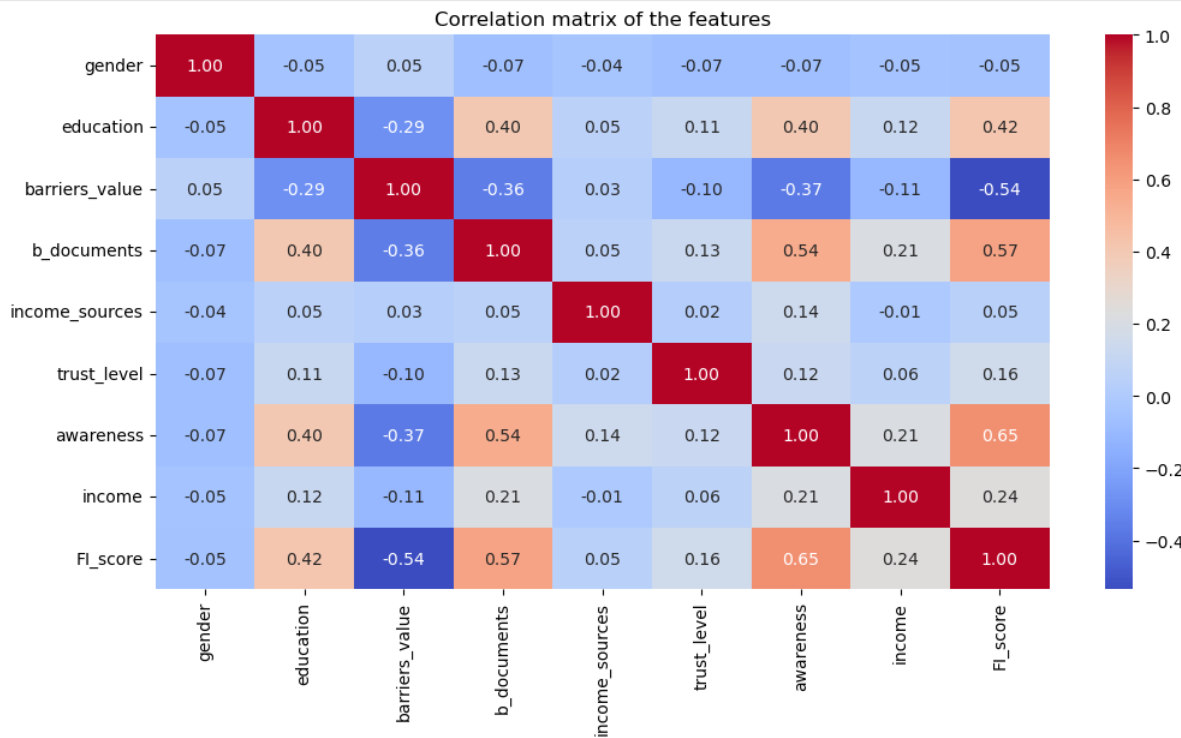
\includegraphics[scale=0.35]{Screenshot 2025-08-15 101706.png} 

\end{frame}


% Challenges
\begin{frame}{Challenges for Young People (15--24 years)}
\begin{itemize}
    \item Limited awareness of financial services and digital payment methods
    \item Lack of required banking documents (e.g., ID, proof of address)
    \item Gaps in financial literacy and education
    \item Low trust in financial institutions
    \item Limited income sources and irregular earnings
\end{itemize}
\end{frame}

% Opportunities
\begin{frame}{Opportunities for Improvement}
\begin{itemize}
    \item Financial literacy programs in schools and communities
    \item Simplified KYC processes to make account opening easier
    \item Youth-focused digital banking products (mobile money, e-wallets)
    \item Trust-building initiatives through transparent communication
    \item Partnerships between banks, fintech, and youth groups
\end{itemize}
\end{frame}

% Conclusion
\begin{frame}{Conclusion}
\begin{block}{Key Findings}
Analysis indicates that:
\begin{enumerate}
    \item \textbf{Awareness \& Use of Financial Services}
    \item \textbf{Possession of Banking Documents}
    \item \textbf{Educational Literacy}
\end{enumerate}
are the most significant factors influencing financial inclusion among young people.
\end{block}
\end{frame}

\begin{frame}
\begin{block}{}
\begin{center}
Thank you for listening...
\end{center}
\end{block}
\end{frame}

\end{document}
